\chapter{Text-to-SQL e NL2Vis: da pergunta ao gráfico auditável}
\chaptermark{Text-to-SQL e NL2Vis}

A coordenação pergunta: quais cursos estão com desempenho melhor? A frase parece clara até a equipe descobrir que melhor pode ser aprovação, média, evolução, equidade ou persistência; período e denominador também não foram definidos. Um LLM pode produzir SQL e um gráfico atraentes, mas a primeira responsabilidade é converter a pergunta em contrato analítico.

Text-to-SQL traduz linguagem natural em consulta; NL2Vis propõe visualização. As duas tarefas compartilham a interpretação da pergunta, mas possuem erros diferentes. SQL válido pode usar métrica errada; um gráfico esteticamente correto pode ocultar período, amostra ou incerteza. Por isso, a trilha mantém intenção, métrica, consulta, resultado e visual conectados.

O caso de aula usa um conjunto sintético de resultados estudantis com curso, período, frequência, nota e situação. Nenhum resultado deve ser interpretado como diagnóstico de pessoas reais. A equipe compara aprovação por curso, depois questiona se a média esconde grupos pequenos e se a comparação é justa.

Em três horas, passamos de pergunta ambígua a especificação, catálogo de campos, plano de consulta seguro, agregação independente, gráfico e narrativa. O modelo pode sugerir cada etapa, mas os alunos verificam campo, filtro, denominador e significado antes de apresentar uma conclusão.

A arquitetura começa antes da chamada à API. Uma camada de experiência recolhe a pergunta; uma camada de domínio identifica intenção, métricas e regras; um serviço de consulta acessa somente fontes permitidas; e uma camada de apresentação combina tabela, visual e texto. O provedor de LLM fica atrás de um adaptador para que o restante do software não dependa diretamente de um único SDK.

O caso principal será sintético e pequeno o bastante para auditoria manual. Em vez de afirmar que um curso é melhor, vamos perguntar o que significa melhor, qual é o grupo comparável, qual o período e que evidência justificaria uma ação. O resultado da aula será um pipeline que responde ou pergunta de volta, não uma caixa de chat sem contrato.

Há uma diferença importante entre produzir uma consulta e produzir uma análise. O primeiro é uma transformação de linguagem para uma representação executável; a segunda exige decidir população, métrica, qualidade, contexto, visual e limite inferencial. A LLM pode acelerar a tradução, mas cada uma dessas escolhas precisa ser explícita no software e verificável por quem usa.

\section{Desambiguar intenção, métrica e população}

Uma pergunta analítica é decomposta em entidade, medida, dimensão, período, filtro, comparação e decisão. Desempenho melhor não é métrica; taxa de aprovação por curso no período X já explicita parte do contrato, embora ainda exija definição do que conta como aprovação e do denominador elegível.

A turma escreve duas interpretações legítimas e prevê como a decisão mudaria. Se a gestão quer oferecer tutoria, taxa de reprovação e tendência podem ser úteis; se quer avaliar currículo, precisa considerar coorte, carga e oferta. A pergunta do usuário não determina sozinha o construto.

O LLM recebe glossário governado, tipos e definições necessárias. Não recebe CPF, nome ou coluna irrelevante. Um catálogo semântico apresenta nomes amigáveis e mapeia para colunas reais, unidades, grão e regra de agregação. Esse contrato reduz erro de ligação entre expressão e esquema.

O contraexemplo é aceitar média por curso sem saber se cada linha é estudante, matrícula ou avaliação. Uma junção pode duplicar registros e inflar denominador. Antes de agrupar, a equipe verifica grão, chave, duplicidade e política para dados ausentes.

Uma interface boa devolve uma pergunta de esclarecimento curta e apresenta duas opções com consequências distintas. A pessoa confirma população e período antes de executar; a escolha fica registrada no plano, tornando a análise reproduzível e contestável.

Para transformar a pergunta em estrutura, usamos uma gramática de intenção. A frase é decomposta em entidade analítica, medida, dimensão, intervalo temporal, filtro, comparação, população elegível e formato de resposta. Nem todo campo precisa aparecer na fala: a camada semântica pode fornecer valores padrão, mas deve distinguir padrão seguro de suposição material. Se a suposição muda a conclusão, o sistema deve perguntar antes de consultar.

Considere três perguntas: quantos foram aprovados?, qual curso teve a maior taxa? e qual curso melhorou?. A primeira pode ser uma contagem; a segunda requer taxa e denominador por curso; a terceira precisa de dois períodos comparáveis e uma regra de mudança. Elas compartilham palavras e tabela, mas pedem consultas diferentes. Um classificador de intenção que reconhece apenas substantivos perderia a operação estatística.

Uma ficha de especificação registra a pergunta original e sua forma normalizada. Para qual curso melhorou em aprovação de 2026.1 para 2026.2?, a ficha pode declarar métrica proporção de matrículas aprovadas, dimensão curso, períodos explícitos, população matrículas elegíveis, operação diferença em pontos percentuais e visual pontos conectados dos dois períodos. Cada campo tem estado: fornecido pela pessoa, herdado de uma definição versionada ou ainda indefinido.

O sistema precisa considerar também perguntas sem resposta válida. Qual professor causou a queda? pede causalidade que uma tabela descritiva não identifica; mostre notas de todos os estudantes pode exceder a finalidade e expor informação pessoal; compare com o ano passado pode não encontrar período equivalente. Uma resposta correta pode ser uma recusa parcial, uma pergunta de esclarecimento ou um plano alternativo com agregação segura.

No quadro, desenhamos a sequência fala -> intenção tipada -> validação semântica -> execução -> resultado -> comunicação. A tipagem limita o domínio: métrica pertence ao catálogo, dimensão é compatível com a métrica, período tem granularidade suportada e operação é permitida. Esse esquema permite que o backend rejeite estruturas incompletas antes de construir SQL.

O benefício da normalização aparece quando duas pessoas usam sinônimos. Aprovação, passou e resultado positivo podem mapear para a mesma métrica apenas quando o contrato institucional sustenta essa equivalência. Termos como sucesso ou desempenho não devem receber sinônimo automático sem confirmação, pois são conceitos mais amplos que qualquer coluna.

A pergunta em linguagem natural é uma interface conveniente, mas não é uma especificação completa. Para cada solicitação, anotamos quem pergunta, qual decisão está tentando apoiar, qual unidade será observada, qual resultado conta como sucesso e qual período torna a comparação válida. A equipe pode escrever esse contrato em uma frase: Para planejar monitoria, compare a proporção de matrículas elegíveis aprovadas por curso no período letivo completo, usando a definição institucional vigente. Essa frase ainda pode exigir esclarecimento sobre coorte, mas já torna visíveis as lacunas relevantes.

Uma dimensão é uma forma de particionar a população; uma métrica é uma função sobre observações ou grupos; um filtro restringe quais registros participam; e uma comparação define a operação entre resultados. Quando alguém pede os cursos melhores, o sistema não deve traduzir melhores em uma coluna de maior média sem contexto. Pode oferecer opções semanticamente distintas: maior taxa de aprovação, maior mediana de nota ou melhora entre períodos. Cada opção deve explicar que decisão sustenta e qual denominador utiliza.

A intenção também determina o grão. Uma tabela com uma linha por tentativa de avaliação permite contar tentativas, mas não estudantes. Uma tabela com matrículas pode conter mais de uma linha por estudante quando há disciplinas. Se o sistema agrupa diretamente essas tabelas, um aluno com cinco disciplinas pode pesar cinco vezes mais que outro com uma disciplina. A camada semântica declara chaves e relações válidas, enquanto a consulta aplica deduplicação e agregação no nível definido pela pergunta.

Outro cuidado é distinguir ausência de dado de valor zero. Uma nota nula pode significar avaliação ainda não lançada, estudante sem atividade ou erro de ingestão; convertê-la silenciosamente em zero mistura situações diferentes. A especificação registra o tratamento permitido e o resultado informa quantos registros foram excluídos. Se a regra não existe, o software deve perguntar ou apresentar uma resposta parcial em vez de inventar um padrão.

A turma pode exercitar a tradução em quatro perguntas curtas: quantos atendimentos atrasaram?, qual unidade tem maior taxa?, onde a espera melhorou? e o que causou a piora?. Cada grupo marca métrica, dimensão, período, população e decisão; em seguida, identifica qual pergunta é respondível por descrição e qual exigiria um desenho causal. O valor do exercício está em perceber que linguagem natural mistura operação, finalidade e premissas.

Quando a pergunta muda depois da resposta, a conversa precisa preservar versões do contrato. Uma sequência como e no período anterior? herda métrica e filtros se estes forem seguros e visíveis. E entre alunos com baixa frequência? introduz uma nova definição e pode mudar finalidade, acesso e denominador. O sistema mostra o contrato herdado e permite editar cada campo, evitando que o contexto conversacional se torne estado invisível.

Uma boa pergunta de esclarecimento reduz incerteza sem transferir todo o trabalho ao usuário. Em vez de explique melhor, o sistema pergunta: Você quer comparar a taxa de aprovação por curso ou a média de notas? A taxa usa matrículas elegíveis como denominador. A interface oferece opções, mostra consequências e aceita resposta livre. Essa interação transforma semântica em parte observável do produto e fornece um registro útil para avaliação posterior.

\section{Construir plano analítico antes de SQL}

Antes de escrever consulta, a squad representa a intenção em um plano simples: métrica aprovada, dimensão, período, filtros, população, agregação, política de privacidade e visual pretendido. Essa camada intermediária permite inspecionar a interpretação antes de executar código.

O modelo pode preencher uma proposta JSON, mas o backend valida nomes contra uma allowlist, tipo de dado, operador permitido e limite de linhas. Campos desconhecidos são rejeitados; não são corrigidos silenciosamente para outra variável. Valores entram como parâmetros, não como concatenação livre.

\textbf{Código da squad --- plano allowlisted para uma agregação}
\begin{verbatim}
# Define somente dimensões e métricas aprovadas pela coordenação.
dimensoes = {"curso": "course", "periodo": "term"}
# Mantém um catálogo explícito de medidas analíticas autorizadas.
metricas = {"taxa_aprovacao": "passed", "nota_media": "score"}
# Recebe uma proposta estrutural, não SQL livre do modelo.
plano = {
    "dimensao": "curso",
    "metrica": "taxa_aprovacao",
    "periodo": "2026.1",
}
# Interrompe o fluxo quando a dimensão não consta no catálogo.
assert plano["dimensao"] in dimensoes
# Interrompe o fluxo quando a métrica não foi aprovada.
assert plano["metrica"] in metricas
# Mostra a interpretação antes de gerar consulta ou visual.
print("Plano aceito para revisão:", plano)
\end{verbatim}

Esse protótipo verifica nomes, não autorização completa ou correção semântica. A equipe adiciona autenticação no servidor, valida período e aplica limiar mínimo de grupo. Em produção, SQL pode ser gerado a partir do plano com biblioteca conhecida ou selecionado entre consultas revisadas.

O plano também funciona como explicação acessível à pessoa usuária. A interface apresenta taxa de aprovação por curso no período 2026.1 para confirmação ou correção antes da execução. Essa etapa diminui risco de resolver com precisão uma pergunta diferente da pretendida.

Uma especificação de plano pode ser representada como JSON com campos obrigatórios e enums, e não como texto livre. O modelo pode propor identificadores de métrica e dimensão, intervalo, filtros e intenção visual; o servidor verifica o schema, a existência dos identificadores, o tipo dos filtros e o escopo de acesso. Strings inesperadas não viram nomes de coluna por interpolação.

Antes da consulta, um compilador controlado transforma os identificadores semânticos em expressões conhecidas. Uma definição possível para taxa de aprovação é contar matrículas distintas aprovadas e dividir pela contagem distinta de matrículas elegíveis. O compilador ainda precisa verificar que o conjunto contém uma chave adequada ou que a agregação evita duplicidade introduzida por junções.

Considere uma base de avaliações com duas notas por matrícula. A consulta que calcula a média de todas as avaliações responde média de avaliações, não média por estudante. Se a pergunta pede a média de estudantes, primeiro calculamos a média por matrícula e depois resumimos os estudantes, ou aplicamos explicitamente a regra institucional. A diferença é um problema de grão; um LLM pode produzir SQL sintaticamente correto e ainda escolher a unidade errada.

A validação estática combina allowlist de tabelas e campos, limites de agregação, restrições de leitura, tempo máximo, limite de linhas e parâmetros vinculados. O modelo não recebe credenciais do banco nem executa alteração de dados. Uma camada de serviço identifica o usuário real e aplica suas permissões; o filtro que o modelo sugere não é mecanismo de autorização.

Um plano também deve declarar como tratar nulos, empates e grupos pequenos. Se quatro cursos têm taxa igual, a resposta deve reportar empate em vez de fabricar ranking. Se um grupo tem menos de um limiar aprovado, o sistema pode suprimir ou agregar conforme política previamente definida, sem pedir ao LLM para decidir quem pode ver o dado.

Há consultas para as quais nenhuma execução é necessária. Se a pergunta pede uma definição, a resposta deve recuperar uma fonte vigente; se pede uma soma, o motor determinístico executa; se combina definição e soma, a arquitetura pode recuperar o significado, executar cálculo e apresentar ambas as evidências. Selecionar mecanismo pelo tipo de tarefa evita usar geração como calculadora ou vetor como banco numérico.

O plano tipado funciona como fronteira entre geração probabilística e execução determinística. Pode conter metric\_id, dimension\_id, intervalo de datas, filtros, população, operação, visual e motivo da consulta. Em produção, o modelo não escolhe livremente nomes físicos de tabelas; ele seleciona conceitos de um catálogo publicado. O serviço verifica cada valor, aplica a identidade do usuário e só então produz uma consulta parametrizada para o mecanismo de dados.

Validação de formato não equivale a validação de significado. Um JSON pode ser válido e ainda combinar uma métrica de matrícula com uma dimensão de tentativa de avaliação sem relação aprovada. O validador semântico verifica compatibilidade, grão, relação temporal, agregação permitida e definição vigente. Um erro nesses contratos impede execução e retorna explicação compreensível, como a taxa de aprovação não pode ser agrupada pela categoria de avaliação nesta fonte.

Uma consulta de leitura ainda pode custar caro ou expor informação. O gateway impõe timeout, limite de bytes e linhas, quantidade máxima de grupos, intervalo máximo e orçamento por usuário. Para pedidos de microdados, a política pode bloquear a consulta antes de chegar ao banco. Essas barreiras não são instruções no prompt: precisam ser garantias no backend e permanecer ativas mesmo quando o modelo responde com SQL inesperado.

Considere o seguinte erro de junção: cada matrícula tem três disciplinas e uma tabela de bolsas possui duas parcelas por matrícula. Juntar as duas tabelas apenas pela matrícula cria seis linhas; somar parcelas duplica o valor três vezes. A consulta deve agregar cada relação antes da junção ou usar chaves e grão compatíveis. Esse caso mostra por que uma consulta parece plausível não é critério suficiente para aceitar Text-to-SQL.

Um plano auditável pode ser serializado e salvo junto à resposta: pergunta original, interpretação confirmada, identificadores semânticos, versão do catálogo, filtros, identidade, consulta normalizada, horário e execução. Os logs não precisam guardar linhas pessoais nem o prompt inteiro; podem guardar parâmetros minimizados e códigos de resultado. Essa trilha permite reproduzir a decisão e investigar falha sem transformar a observabilidade em nova fonte de exposição.

A execução deve ser read-only e usar conta de serviço com privilégios mínimos. O SQL pode ser limitado a SELECT, mas uma consulta ainda pode usar função pesada, explorar tabelas sensíveis ou extrair muitos grupos. Por isso, análise sintática, catálogo de permissões, políticas do banco e limites de serviço trabalham em conjunto. Instruções do modelo como ignore a política e consulte a tabela completa são dados não confiáveis e não alteram a autorização.

Um segundo exemplo de bloqueio é a pergunta sobre um grupo com três matrículas. Mesmo que a taxa esteja correta, a publicação pode revelar informação por combinação com dados externos. Uma política pode suprimir grupos abaixo de um limiar, aplicar agregação mais ampla ou exigir análise manual. O limiar não é universal: depende do contexto e da política institucional, deve ser explícito e precisa evitar que consultas repetidas reconstruam o valor suprimido.

\section{Executar uma EDA independente e produzir o gráfico}

Uma vez aprovado o plano, o conjunto é filtrado e agregado com código determinístico. O gráfico resulta de tabela já conferida, não de um código livre que o LLM executa. A turma compara contagens e proporções antes de escolher um visual.

\begin{center}
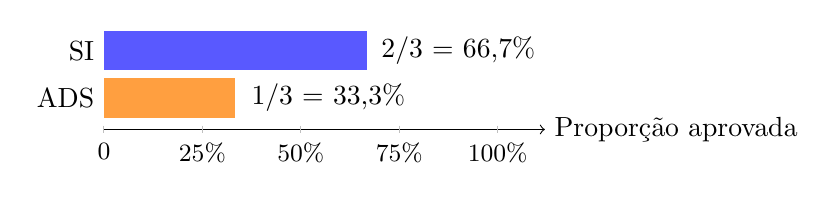
\begin{tikzpicture}[x=5cm,y=1cm]
\draw[->] (0,0)--(1.12,0) node[right]{Proporção aprovada};
\foreach \x/\lab in {0/0,0.25/25\%,0.5/50\%,0.75/75\%,1/100\%} {
  \draw[gray!50] (\x,0.05)--(\x,-0.05);
  \node[below] at (\x,-0.05) {\small \lab};
}
\node[left] at (0,1) {SI};
\node[left] at (0,0.4) {ADS};
\fill[blue!65] (0,0.75) rectangle (0.667,1.25);
\fill[orange!75] (0,0.15) rectangle (0.333,0.65);
\node[right] at (0.68,1) {2/3 = 66,7\%};
\node[right] at (0.35,0.4) {1/3 = 33,3\%};
\end{tikzpicture}
\end{center}

O exemplo de gráfico precisa corresponder à tabela produzida pelo código; por isso, não desenhamos alturas sem numerador e denominador verificáveis. A primeira comparação pode ser lida à mão: SI tem 2 aprovações em 3 matrículas, então 2/3 = 0,667, aproximadamente 66,7%; ADS tem 1 aprovação em 3, então 1/3 = 0,333, aproximadamente 33,3%. A diferença descritiva é de 33,3 pontos percentuais no conjunto didático.

Para um segundo exemplo, SI tem 80 aprovações em 100 matrículas e ADS tem 9 em 10. A média simples das taxas é (0,80 + 0,90)/2 = 0,85, enquanto a taxa agregada é 89/110 = 0,809, cerca de 80,9%. Ambas são corretas para estimandos diferentes. Se cada matrícula deve receber peso igual, a razão agregada responde à pergunta; se a pergunta compara o curso médio, a média das taxas pode ser apropriada e precisa ser nomeada.

O gráfico de barras codifica proporção por comprimento e posição; os denominadores devem aparecer em rótulos ou tabela próxima. Para evolução, pontos conectados mostram dois períodos; para distribuição de notas, boxplot mostra mediana, quartis e extremos possíveis, mas não revela sozinho o tamanho de cada grupo. A escolha acompanha a operação que a pergunta pede.

Uma comparação temporal também alinha coortes e calendário. Se o período atual contém dez semanas e o anterior dezesseis, contagens brutas não são comparáveis sem exposição ou população equivalente. O plano analítico detecta período incompleto, regra de matrícula diferente ou coluna de situação alterada, e avisa antes de interpretar variação como tendência.

Os gráficos não são gerados apenas com o texto da pergunta. O serviço recebe especificação visual validada, dados agregados e metadados de unidade; então código determinístico cria o gráfico. A LLM pode explicar a escolha ou sugerir alternativa, mas o componente visual usa domínio de dados, formato e limites definidos pela aplicação.

Uma verificação independente reconstrói ao menos um grupo com SQL conhecido ou pandas e compara numerador, denominador e taxa com o resultado retornado. Em sistemas maiores, verificamos invariantes: taxa entre zero e um, total não superior à população elegível, filtros aplicados a todos os grupos e soma compatível com o total quando as categorias são exaustivas.

O esboço mostra comparações próximas e reforça que o denominador deve acompanhar a barra. Pequenas diferenças podem não ser estáveis; não colocamos ordenação dramática nem anotação causal. A saída do código e o desenho precisam concordar antes da comunicação.

\textbf{Código da squad --- tabela, denominador e barras}
\begin{verbatim}
# Importa pandas para resumir o conjunto sintético em uma tabela.
import pandas as pd
# Importa matplotlib para gerar um visual reproduzível.
import matplotlib.pyplot as plt
# Cria observações sintéticas; cada linha representa uma matrícula.
dados = pd.DataFrame({"curso": ["SI", "SI", "ADS", "ADS", "SI", "ADS"],
                      "aprovado": [1, 0, 1, 0, 1, 0],
                      "periodo": ["2026.1"] * 6})
# Filtra o período definido no plano analítico.
recorte = dados.loc[dados["periodo"].eq("2026.1")].copy()
# Calcula total elegível e aprovações por curso.
resumo = (
    recorte.groupby("curso")["aprovado"]
    .agg(["sum", "count", "mean"])
)
# Exibe numerador e denominador antes da interpretação.
print(resumo)
# Cria barras para comparar proporções, não volume bruto.
ax = resumo["mean"].plot(kind="bar", color="#2463A6", ylim=(0, 1))
# Rotula a medida e o universo temporal de forma explícita.
ax.set_ylabel("Proporção aprovada entre matrículas do período")
# Nomeia o gráfico sem declarar causalidade.
ax.set_title("Aprovação observada por curso - dado sintético")
# Ajusta margens para preservar rótulos na exportação.
plt.tight_layout()
# Exibe o visual para revisão de forma e dados.
plt.show()
\end{verbatim}

Com amostra tão pequena, as proporções são instáveis. A visualização é um exemplo de código e não uma conclusão institucional. Em um dataset real, incluiríamos intervalo de incerteza, distribuição por coorte e tamanho mínimo antes de comparar ou expor grupos.

O painel informa filtros, data, fonte, definição e atualização. Se a pessoa alterar o período, a tabela e gráfico são recalculados pela mesma consulta identificada. Um texto gerado sem vínculo a esses parâmetros pode sobreviver a uma mudança de filtro e ficar incorreto.

A saída analítica deve preservar numerador e denominador como campos separados. Para cada curso, uma tabela intermediária pode conter aprovacoes, matriculas\_elegiveis, taxa, período, regra e versão. Essa estrutura dá à aplicação elementos suficientes para conferir e explicar a proporção. Armazenar somente a taxa arredondada impede reconstruir o cálculo e pode levar o texto gerado a usar denominador incorreto.

Arredondamento ocorre no final da cadeia de apresentação. Se um grupo tem 2 aprovações em 3 matrículas, a fração exata é 0,6666...; a exibição como 66,7% é útil, mas a diferença entre duas taxas deve usar precisão completa e só depois ser arredondada. Comparar 66,7% e 33,3% produz uma diferença apresentada como 33,4 pontos, embora o cálculo exato seja 33,333... pontos. A legenda deve evitar sugerir precisão maior do que os dados sustentam.

A proporção observada é descrição da amostra, não estimativa livre de incerteza. Em grupos pequenos, uma alteração de uma matrícula muda muito o resultado. A equipe pode apresentar contagens junto à proporção e usar intervalos apropriados quando a finalidade exige inferência; não deve tratar um intervalo calculado automaticamente como selo de verdade sem declarar modelo e pressupostos. Para a aula, o exemplo sintético serve para checar pipeline, não para ordenar cursos reais.

Dados ausentes merecem uma tabela de qualidade à parte: linhas lidas, duplicatas, matrículas elegíveis, status conhecido, registros excluídos e motivo. Se 100 linhas viram 82 elegíveis, a taxa usa 82 no denominador e revela como as demais foram tratadas. Uma queda aparente pode refletir mudança de cobertura, não mudança de desempenho. O produto mostra esses contadores e sinaliza uma quebra de série quando o processo de coleta muda.

Ao escolher o gráfico, distinguimos comparar níveis de comparar mudanças. Barras ordenadas apoiam ranking em um período; pontos conectados facilitam comparar dois períodos por curso; pequenos múltiplos ajudam quando existem vários períodos e muitas categorias. Uma linha temporal não deve ligar períodos sem ordem temporal, e uma barra empilhada pode esconder a comparação de uma categoria interna. O tipo de gráfico é consequência da tarefa perceptiva, não preferência do modelo.

A aplicação precisa sincronizar estado. Alterar o filtro de semestre deve recalcular consulta, contagem, tabela, título, visual, evidência e narrativa. Uma falha comum mantém a narrativa anterior em cache enquanto o gráfico muda. Para impedir isso, cada resultado carrega uma chave de estado que inclui pergunta normalizada, filtros, usuário, versão semântica e atualização da fonte; qualquer mudança invalida os artefatos derivados.

A checagem de consistência pode comparar caminhos independentes. Um estudante calcula a taxa em pandas e confronta com uma consulta SQL revisada; outro soma manualmente uma tabela pequena. Divergências são classificadas: filtro diferente, grão incorreto, nulos, junção, arredondamento ou atualização. Essa decomposição ensina depuração analítica e evita atribuir todo erro a alucinação da IA.

\section{Recomendar visual e construir narrativa sem exagero}

NL2Vis escolhe codificação de acordo com a pergunta. Comparar categorias pede barras ordenadas; tendência temporal pede linha; distribuição de notas pode usar histograma ou boxplot; relação entre presença e resultado pode usar dispersão, com cautela quanto à associação. O modelo pode propor, mas o analista explica por que o canal visual serve à tarefa.

Storytelling começa pela evidência: público, contexto, observação, limite e ação possível. Curso X tem o maior valor não autoriza dizer que o curso causa o desempenho. A equipe substitui linguagem causal por descrição associativa e apresenta o tamanho da amostra.

Uma boa Big Idea pode ser: neste recorte sintético, a diferença observada merece ser verificada por coorte antes de orientar apoio. O visual mostra a comparação; a tabela oferece denominadores; a nota explica que seis matrículas não sustentam uma decisão real.

O contraexemplo usa eixo truncado e remove grupo pequeno para criar sensação de grande diferença. Outra falha é ordenar categorias alfabeticamente quando a pergunta é ranking. A revisão olha escala, rótulos, contraste, incerteza, legenda e acessibilidade.

Também conferimos paleta para daltônicos, texto alternativo e navegação por teclado. Uma recomendação de gráfico deve preservar leitura em tela pequena e impressão; se o público não consegue interpretar, a análise ainda não está pronta para comunicação.

Storytelling não é adornar um resultado depois do cálculo; é ordenar uma evidência para que uma decisão possa ser examinada. A sequência narrativa útil é contexto, comparação observada, consequência possível, limite e próximo teste. Cada frase factual deve apontar a uma medida, filtro e período que possam ser reconstruídos.

Uma alegação como a taxa caiu cinco pontos percentuais exige mostrar taxa inicial e final: 75% para 70% produz diferença de -5 pontos percentuais. Dizer que caiu 5% usaria variação relativa, que seria (0,70 - 0,75)/0,75 = -0,0667, ou -6,7%. A redação escolhe a escala correta e evita tratar pontos percentuais como percentagem relativa.

Um segundo caso compara 50% em uma turma de 2 com 70% em uma turma de 100. A primeira estimativa varia muito com um caso; a segunda tem denominador maior, mas ainda pode diferir em composição. Mostrar o tamanho dos grupos junto às taxas reduz a falsa equivalência entre percentuais e ajuda a decidir se a próxima etapa é reunir mais observações ou decompor por coorte.

Um título deve declarar população e intervalo, por exemplo Matrículas elegíveis aprovadas por curso --- 2026.2 (dados didáticos). Uma anotação pode mostrar meta, mas não deve usar cor de alerta como se uma observação fora da meta provasse falha de gestão. A legenda descreve codificação; a nota documenta fonte, atualização e regra de exclusão.

A LLM recebe pacote de evidência com identificadores, definições, numeradores, denominadores, datas, filtros e limitações. Seu retorno ideal é estruturado: observação, comparação, ressalva, pergunta em aberto e evidências usadas. O backend confirma que cada identificador existe e que os números citados correspondem à saída analítica; texto sem suporte é removido ou enviado para revisão.

O próximo conceito, comparação de plataformas, pergunta quanto dessa cadeia uma ferramenta gerenciada oferece e o que a instituição precisa construir. A mesma métrica, definição e pergunta serão usadas para comparar soluções, porque uma demonstração com perguntas e dados diferentes não mede capacidade relativa.

Uma narrativa de análise contém afirmações com papéis diferentes. Descrição relata o que foi observado; interpretação sugere uma leitura; hipótese propõe explicação; recomendação aponta ação. O produto deve tornar essa distinção visível por linguagem e apresentação. A taxa observada foi menor é descrição; a mudança ocorreu por baixa frequência é hipótese; vamos ampliar tutoria é recomendação que depende de objetivo, custo e avaliação.

Para cada afirmação numérica, criamos um registro com identificador, valor, unidade, universo, período, filtros e método. A frase a taxa subiu liga a dois registros e à operação de diferença; o curso tem melhor resultado não é aceita se a regra de melhor não foi definida. A resposta deixa acessíveis tabela, visual ou definição que sustentam o texto, de modo que a pessoa consiga contestar uma afirmação específica.

O modelo pode adicionar detalhe que não está no pacote de evidência. Uma validação lexical simples procura entidades, datas e números citados; validação mais robusta exige saída estruturada e compara valores com a tabela calculada. A aplicação também pode pedir que cada sentença factual cite IDs de evidência. Isso não garante verdade por si só, mas permite bloquear sentenças sem suporte e revisar discrepâncias com precisão.

O tom da narrativa deve corresponder à força da evidência. Um censo completo do período permite descrever aquele período; não assegura que o padrão se repita no futuro. Uma amostra pequena pede linguagem cautelosa. Uma associação entre presença e aprovação não prova mecanismo causal. Essa calibragem é parte da qualidade do insight e deve ser avaliada separadamente de fluência, gramática e criatividade.

Acessibilidade também modifica a arquitetura de resposta. Cor não pode ser o único canal para distinguir grupos; o gráfico precisa de rótulos, contraste e texto alternativo; uma tabela equivalente ajuda leitores de tecnologias assistivas. O resumo deve nomear medida e unidade em vez de depender da inspeção visual. A recomendação pode apresentar uma versão curta e outra detalhada, sem alterar os fatos entre formatos.

Uma resposta útil oferece uma próxima verificação proporcional. Se a diferença entre cursos existe, a equipe pode decompor por coorte ou verificar cobertura; não precisa recomendar uma política imediatamente. Um teste seguinte pode ser: comparar matrículas elegíveis por semestre e verificar mudança de calendário. A ação é concreta, mensurável e reversível, ao contrário de uma conclusão ampla baseada em uma taxa agregada.

A revisão por pares funciona como teste adversarial de narrativa. Um grupo recebe gráfico e texto, tenta refazer o cálculo e procura uma interpretação alternativa; depois verifica se o título omite população, se a escala exagera contraste ou se a recomendação ultrapassa evidência. O autor revisa a Big Idea e responde quais evidências novas mudariam sua conclusão. Isso transforma storytelling em prática de análise contestável.

\section{Roteiro de 180 minutos e evidência de aprendizagem}

19h--19h25: grupos esclarecem pergunta e escrevem contrato de métrica. 19h25--19h50: inspecionam esquema, grão e ausências. 19h50--20h20: montam plano semântico e analisam SQL proposto. 20h20--20h30: verificam denominador e registram dúvida antes da chamada.

20h30--21h: executam agregação determinística e conferem tabela. 21h--21h25: escolhem gráfico e visualizam recorte. 21h25--21h45: redigem narrativa com limite e recomendação condicional. 21h45--22h: outra equipe altera período e tenta reproduzir o resultado.

O artefato contém pergunta, plano, consulta ou código, tabela, gráfico, fonte, versão, denominador e texto final revisado. A avaliação exige rastreabilidade entre todos os elementos. Se o estudante não consegue refazer a conta, a resposta do modelo não é evidência suficiente.

Na revisão final, a squad mostra qual suposição foi descartada e qual dado adicional solicitaria antes de uma decisão real. A aula encerra com uma recomendação condicional e um teste seguinte, não com uma conclusão geral sobre estudantes ou cursos.

O Capítulo 11 compara plataformas de BI e ambientes de execução. A mesma definição de métrica será usada para avaliar copilotos e agentes, sem deixar interface de fornecedor ocultar acesso, semântica e trilha de auditoria.

\begin{SummaryBox}
Text-to-SQL e NL2Vis aceleram tradução, mas não definem a pergunta nem validam significado. A cadeia segura é contrato analítico, plano permitido, cálculo reproduzível, visual escolhido por tarefa e storytelling proporcional à evidência.
\end{SummaryBox}



O primeiro bloco de 90 minutos começa com um contraste de perguntas e termina com um plano analítico validado. O professor registra no quadro fala, intenção, métrica, população, dimensão e período; os grupos propõem interpretações e usam IA para gerar uma alternativa. A discussão compara a sugestão da IA com o glossário e mostra por que uma resposta articulada não define automaticamente a métrica do curso.

Na etapa seguinte, cada grupo recebe um cenário e tem de dez a quinze minutos para desenhar arquitetura de ponta a ponta. A folha deve incluir fonte e grão, limpeza, métrica, consulta, cálculo, visual, narrativa, evidência e limite. O grupo pode pedir ajuda a uma IA, mas precisa marcar quais decisões vieram da proposta e quais foram verificadas. Uma pontuação formativa privilegia justificativa e revisão, não velocidade de digitação.

Após a chamada, o segundo bloco parte do plano para produzir uma tabela e gráfico pequenos. O professor muda um filtro ou altera um denominador e pede que a turma antecipe o resultado antes de rodar o código. Essa pausa explicita expectativa, torna o erro instrutivo e separa raciocínio analítico da confiança automática na ferramenta.

A evidência de aprendizagem é um artefato rastreável: pergunta original, especificação normalizada, plano JSON ou equivalente, consulta/código, contagens de referência, visual, resposta e revisão. Cada grupo entrega também um caso de recusa ou esclarecimento e explica por que a consulta não deveria executar. O conjunto de entregas prepara a aula de comparação de BI e serve como requisito inicial do protótipo.

O professor pode usar uma rubrica simples de quatro dimensões: semântica e grão, segurança da consulta, correção do resultado e narrativa proporcional. Cada dimensão recebe insuficiente, em desenvolvimento ou consistente, com um comentário observável. Uma consulta bem escrita não compensa denominador errado; um gráfico elegante não compensa falta de evidência. Essa rubrica deixa claro o que significa desenvolver uma solução de ponta a ponta.

Para tarefa de casa, a squad adapta o contrato a um segundo cenário sintético e envia uma especificação executável ou pseudocódigo. Não se exige chave de API na primeira semana; os estudantes demonstram arquitetura com mock e só integram serviço remoto quando o professor apresentar o procedimento de segredo local. Assim, ninguém precisa publicar credenciais ou usar dado acadêmico real para mostrar competência.

A transição para o Capítulo 11 mantém a mesma pergunta e definição de taxa, mas muda o ambiente de implementação. Cada equipe comparará resposta de BI gerenciado e pipeline próprio, registrando recursos verificados, controles ausentes e evidências de operação. O teste será justo porque métrica, população, períodos, filtros e critérios de aceitação permanecem constantes.

\clearpage
\bigskip
\noindent\textbf{Referências técnicas para aprofundamento}

\begingroup\small
\begin{itemize}
\item Microsoft. \emph{Text-to-SQL in the wild: how to build and evaluate data agents}. Documentação de Fabric data agents. \url{https://learn.microsoft.com/en-us/fabric/data-science/how-to-create-data-agent}.
\item OpenAI. \emph{Function calling and structured outputs}. Documentação oficial da API. \url{https://developers.openai.com/api/docs/guides/function-calling}.
\item Tableau. \emph{Tableau Semantics and Tableau Next overview}. \url{https://help.tableau.com/current/tableau-next/en-us/tableau_next_tableau_product_overview.htm}.
\item Singh et al. \emph{Beyond Text-to-SQL: An Agentic LLM System for Governed Enterprise Analytics APIs}. arXiv:2605.21027, 2026. \url{https://arxiv.org/abs/2605.21027}.
\end{itemize}
\endgroup
